\documentclass{article}
\usepackage{tikz}
\usepackage{bm}
\usetikzlibrary{3d, intersections, decorations.pathmorphing}

\begin{document}

	\begin{tikzpicture}[x={(1cm,-0.4cm)}, y={(1cm,0.4cm)}, z={(0cm,1cm)}]
		% Draw the observer point
		\filldraw (0,0,0) circle (2pt);
		\filldraw (-1,-1,8) circle (1pt);

		\node[right] at (0,0,0) {Observer};

		



		
		% Draw the plane at z=8
		\begin{scope}[canvas is xy plane at z=8, transform shape,shift={(-1,-1,0)}]
			\draw[opacity=0.5] (-2,-2) rectangle (2,2);
			\node at (0, 2.5) {Source Plane};
			% Add a point at the intersection of the line with the plane
			
		\end{scope}
		
		% Draw the reference frame
		\draw[->] (0,0,0) -- (0,0,1) node[right]{$z$};
		\draw[->] (0,0,0) -- (-1,0,0) node[above]{$x$};
		\draw[->] (0,0,0) -- (0,-1,0) node[below]{$y$};
		\draw[->] (0,0,0) -- (-0.95,-0.95, 7.9) node[below left]{$\bm{x}_{\rm true}$};

	\end{tikzpicture}
	
	
	\begin{tikzpicture}[x={(1cm,-0.4cm)}, y={(1cm,0.4cm)}, z={(0cm,1cm)}]
		% Draw the observer point
		\filldraw (0,0,0) circle (2pt);
		\filldraw (-1,-1,8) circle (1pt);

		\node[right] at (0,0,0) {Observer};
		\node[right] at (0,0,6) {$\chi_{\rm LSS}$};

		


		% Draw the vertical line
		\draw[dashed] (0,0,0) -- (0,0,8);
		\node[left] at (0,0,8) {};
		

		
		% Draw the plane at z=8
		\begin{scope}[canvas is xy plane at z=8, transform shape,shift={(-1,-1,0)}]
			\draw[opacity=0.5] (-2,-2) rectangle (2,2);
			\node at (0, 2.5) {Source Plane};
			% Add a point at the intersection of the line with the plane
			
		\end{scope}
		
		% Draw the reference frame
		\draw[->] (0,0,0) -- (0,0,1) node[right]{$z$};
		\draw[->] (0,0,0) -- (-1,0,0) node[above]{$x$};
		\draw[->] (0,0,0) -- (0,-1,0) node[below]{$y$};
		\draw[->, dashed] (0,0,8) -- (-0.95,-0.95,8) node[above right]{$\chi_{\rm LSS} \bm{\theta}_{s}$};
		\draw[->] (0,0,0) -- (-0.95,-0.95, 7.9) node[below left]{$\bm{x}_{\rm true}$};

	\end{tikzpicture}
	
	
	
	
	
	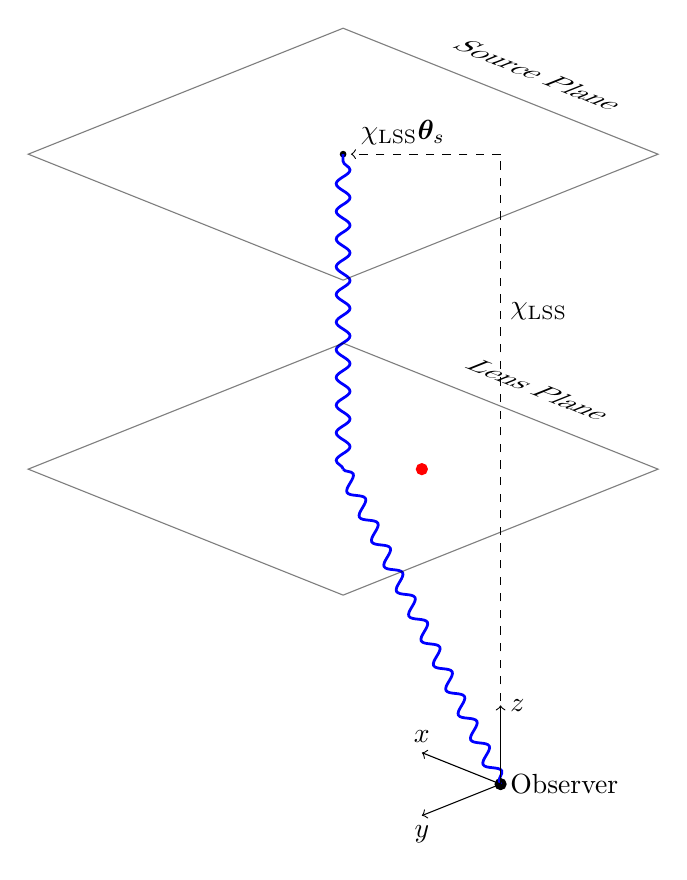
\begin{tikzpicture}[x={(1cm,-0.4cm)}, y={(1cm,0.4cm)}, z={(0cm,1cm)}]
		% Draw the observer point
		\filldraw (0,0,0) circle (2pt);
		\filldraw (-1,-1,8) circle (1pt);
		
		\filldraw[color=red] (-0.5,-0.5,4) circle (2pt);


		\node[right] at (0,0,0) {Observer};
		\node[right] at (0,0,6) {$\chi_{\rm LSS}$};

		


		% Draw the vertical line
		\draw[dashed] (0,0,0) -- (0,0,8);
		
		  \draw[blue, line width=1pt, decorate, decoration=snake] (-1, -1, 4) -- (-1, -1, 8);
		  \draw[blue, line width=1pt, decorate, decoration=snake] (-1, -1, 4) -- (0, 0, 0);

		
		
		% Draw the plane at z=3
		\begin{scope}[canvas is xy plane at z=4, transform shape,shift={(-1, -1, 0)}]
			\draw[opacity=0.5] (-2,-2) rectangle (2,2);
			\node at (0, 2.5) {Lens Plane};

		\end{scope}
		
		% Draw the plane at z=8
		\begin{scope}[canvas is xy plane at z=8, transform shape,shift={(-1,-1,0)}]
			\draw[opacity=0.5] (-2,-2) rectangle (2,2);
			\node at (0, 2.5) {Source Plane};
			% Add a point at the intersection of the line with the plane
			
		\end{scope}
		
		% Draw the reference frame
		\draw[->] (0,0,0) -- (0,0,1) node[right]{$z$};
		\draw[->] (0,0,0) -- (-1,0,0) node[above]{$x$};
		\draw[->] (0,0,0) -- (0,-1,0) node[below]{$y$};
		\draw[->, dashed] (0,0,8) -- (-0.95,-0.95,8) node[above right]{$\chi_{\rm LSS} \bm{\theta}_{s}$};

	\end{tikzpicture}

\
	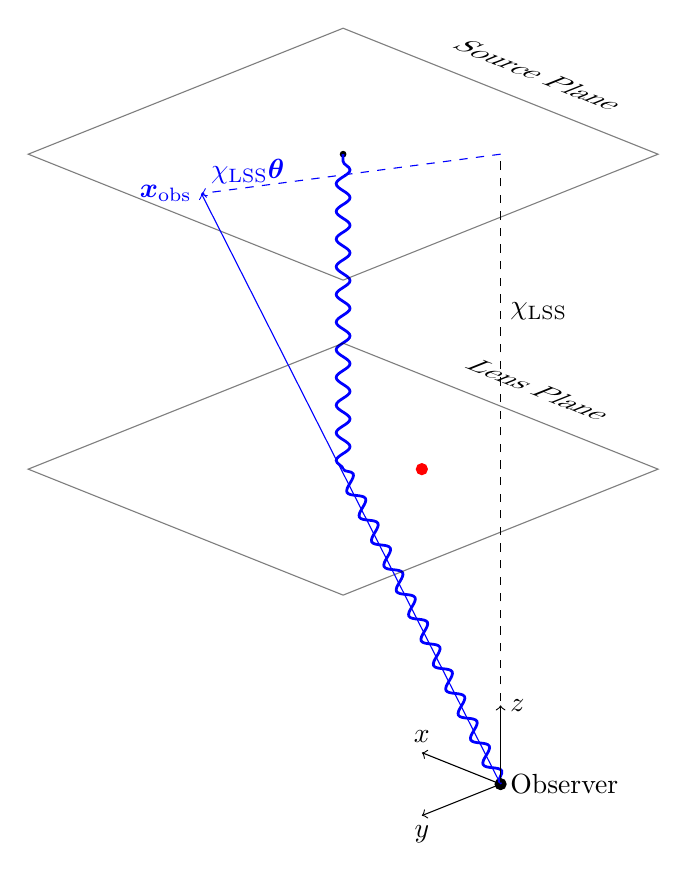
\begin{tikzpicture}[x={(1cm,-0.4cm)}, y={(1cm,0.4cm)}, z={(0cm,1cm)}]
		% Draw the observer point
		\filldraw (0,0,0) circle (2pt);
		\filldraw (-1,-1,8) circle (1pt);
		
		\filldraw[color=red] (-0.5,-0.5,4) circle (2pt);


		\node[right] at (0,0,0) {Observer};
		\node[right] at (0,0,6) {$\chi_{\rm LSS}$};

		


		% Draw the vertical line
		\draw[dashed] (0,0,0) -- (0,0,8);
		
		  \draw[blue, line width=1pt, decorate, decoration=snake] (-1, -1, 4) -- (-1, -1, 8);
		  \draw[blue, line width=1pt, decorate, decoration=snake] (-1, -1, 4) -- (0, 0, 0);

		
		
		% Draw the plane at z=3
		\begin{scope}[canvas is xy plane at z=4, transform shape,shift={(-1, -1, 0)}]
			\draw[opacity=0.5] (-2,-2) rectangle (2,2);
			\node at (0, 2.5) {Lens Plane};

		\end{scope}
		
		% Draw the plane at z=8
		\begin{scope}[canvas is xy plane at z=8, transform shape,shift={(-1,-1,0)}]
			\draw[opacity=0.5] (-2,-2) rectangle (2,2);
			\node at (0, 2.5) {Source Plane};
			% Add a point at the intersection of the line with the plane
			
		\end{scope}
		
		% Draw the reference frame
		\draw[->] (0,0,0) -- (0,0,1) node[right]{$z$};
		\draw[->] (0,0,0) -- (-1,0,0) node[above]{$x$};
		\draw[->] (0,0,0) -- (0,-1,0) node[below]{$y$};
		\draw[->, color=blue, dashed] (0,0,8) -- (-1.9,-1.9,7.5) node[above right]{$\chi_{\rm LSS} \bm{\theta}$};
		\draw[->, color=blue] (0,0,0) -- (-1.9,-1.9,7.5) node[ left]{$\bm{x}_{\rm obs}$};

	\end{tikzpicture}

\


\end{document}
